\chapter{Problemas de Enrutamiento de Vehículos y métodos de búsqueda local}\label{chapter: VRP}

En este trabajo se propone un sistema que permite resolver de manera ágil cualquier de VRP utilizando algoritmos de búsqueda local. En este capítulo se presentan los elementos fundamentales de VRP y de las metaheurísticas de búsqueda local.

En la sección \ref{1-VRPintro} se describen los Problemas de Enrutamiento de Vehículos. En la sección \ref{1-local} se describen los algoritmos de búsqueda local. En \ref{1-Lisp} se presentan algunas características de Common lisp, lenguaje en que se implementó el sistema.

%\newpage

\section{Problema de Enrutamiento de Vehículos}\label{1-VRPintro}
La primera referencia al VRP es \cite{CVRP} y data de 1959. En este trabajo se describe una aplicación real de VRP, entrega de gasolina a varias estaciones de servicio. Para resolverlo, se propone un modelo matemático y una heurística para aproximar la solución.

La versión más sencilla recibe el nombre de CVRP (Capacitated Vehicle Routing Problem) \cite{CVRP} consta de una flota de vehículos que salen de un depósito y deben satisfacer las demandas de una serie de clientes. El objetivo es encontrar una distribución de rutas que se asignan a los vehículos de forma que se optimice determinada métrica (tiempo, combustible, costo total, etc). A partir de esta versión inicial se estudian diversas variantes que se pueden encontrar en la literatura:

\begin{itemize}
	\item VRPTW - VRP con ventanas de tiempo. Cada cliente posee un período de tiempo fijo durante el cual puede ser visitado \cite{VRPTW}.
	\item VRPPD - VRP con recogida y entrega. Los bienes deben ser entregados y recogidos en cantidades fijas \cite{VRPPD}.
	\item MDVRP - VRP con múltiples depósitos. Se cuenta con múltiples depósitos desde los que pueden salir los vehículos \cite{multi}.
	\item VRPB - VRP con backhauls. Los clientes se dividen en dos tipos \textit{A} y \textit{B}. Una solución de este problema debe cumplir con la restricción de que, en todas sus rutas, los clientes de tipo \textit{A} aparezcan antes que los clientes de tipo \textit{B} \cite{backhauls1998}.
\end{itemize}

Los Problemas de Enrutamiento de Vehículos son NP-Duros \cite{2002vehicle}, por lo que las soluciones exactas no son factibles para problemas reales. Para buscar aproximaciones a la solución se utilizan heurísticas y metaheurísticas. En la literatura se reporta \cite{puede} que las metaheurísticas de búsqueda local brindan buenos resultados en poco tiempo y por eso esta es la estrategia seleccionada para este trabajo. A continuación se describen los elementos fundamentales de los algoritmos de búsqueda local.

\section{Metaheurísticas de Búsqueda Local}\label{1-local}
Los algoritmos basados en búsqueda local parten de una solución a la que se llama solución actual y exploran un conjunto de soluciones a las que se les llama vecinos. Las soluciones vecinas se obtienen al aplicar sobre la solución actual un determinado criterio (llamado criterio de vecindad). Cada vecino se analiza y de ellos se escoge uno que puede sustituir o no a la solución actual en dependencia del algoritmo que se esté usando. 

En dependencia de factores como cuántos criterios de vecindad se tiene y cuándo sustituye o no la solución actual, se pueden obtener distintos algoritmos.

Para aplicar cualquier algoritmo de búsqueda local es necesario definir qué es una solución y esto se aborda en la siguiente sección.

\subsection{Representación de soluciones del VRP}\label{1-sol}
Una solución de un Problema de Enrutamiento de Vehículos describe qué clientes visita cada vehículo y en qué orden. Al recorrido de cada vehículo se le llama ruta. Usualmente las rutas se pueden representar por una lista de clientes y las soluciones como una lista de rutas. Por ejemplo, si se define a $P_1$ como un problema clásico (VRP en su versión más simple) que consta de 6 clientes: $[c_1, c_2, c_3, c_4, c_5, c_6]$, entonces una solución $s_1$ se puede definir como:

\begin{equation}
	s_1 = [(c_2,c_3), (c_1,c_4,c_5), (c_6)]
\end{equation}

En $s_1$ se muestra una solución con tres rutas. El vehículo perteneciente a la primera ($r_1$) ruta visita a $c_2$ y $c_3$, el vehículo de la segunda ruta ($r_2$) visita a $c_1$, $c_4$ y $c_5$ y el de la tercera ($r_3$) sólo visita a $c_6$. En todos los casos los recorridos comienzan y terminan en el depósito.

Una vez se definió una solución, es posible definir un criterio de vecindad.

\subsection{Criterios de vecindad}\label{1-criteria}
Un criterio de vecindad es una regla que permite, a partir de una solución actual, obtener nuevas soluciones. En el caso de VRP, estos criterios se pueden formar con modificaciones que se les aplica a los elementos de la solución actual. Algunos de estos criterios de vecindad \cite{Camila, Daniela} pueden ser: 

\begin{enumerate}
	\item Intercambiar dos clientes seleccionados aleatoriamente.
	\item Reubicar un cliente dentro de su ruta en la posición que minimice el costo de esa ruta.
	\item Mover aleatoriamente un cliente de una ruta a otra.
	\item Intercambiar dos vehículos seleccionados aleatoriamente.
\end{enumerate}

Los criterios de vecindad dependen también de la variante del problema sobre la que se trabaje. Por ejemplo, el criterio de \textit{Cambiar vehículos} no tiene sentido para el problema $P_1$ pues en este todos los vehículos son iguales.

Los criterios de vecindad se pueden describir en términos de operaciones elementales. Algunas de ellas son:

\begin{enumerate}
	\item Seleccionar una ruta \texttt{r}. 
	\item seleccionar un cliente \texttt{c} de una posición \texttt{p} de una ruta \texttt{r}.
	\item insertar un cliente \texttt{c} en una posición \texttt{p} de una ruta \texttt{r}.
\end{enumerate}

Las operaciones \textit{Seleccionar ruta}, \textit{seleccionar cliente} e \textit{insertar cliente} se representan en este trabajo con los símbolos \textit{r}, \textit{a} y \textit{b} respectivamente.

Se tiene como ejemplo el criterio \textit{Mover un cliente a cualquier ruta, en cualquier posición}. Este puede ser representado por las operaciones:

\begin{enumerate}
	\item Seleccionar ruta \texttt{$r_x$}.
	\item Seleccionar cliente \texttt{$c_x$} de la posición \texttt{$p_x$} de la ruta \texttt{$r_x$}.
	\item Seleccionar ruta \texttt{$r_y$}.
	\item Insertar cliente \texttt{$c_x$} en la ruta \texttt{$r_y$} en la posición \texttt{$p_y$}.
\end{enumerate}

A partir de un criterio de vecindad y una solución inicial se pueden generar nuevas soluciones vecinas. Un vecino se obtiene asignándole valores específicos a los elementos que forman cada una de las operaciones del criterio. Por ejemplo, a partir de la solución: $s_1 = [(c_2,c_3), (c_1,c_4,c_5), (c_6)]$, se puede obtener un vecino si se usa el criterio (\textit{Mover un cliente a cualquier ruta, en cualquier posición}) con los siguientes valores:

\begin{enumerate}
	\item \texttt{$r_x$} = 1.
	\item \texttt{$c_x$} = \textit{c2}.
	\item \texttt{$p_x$} = 1.
	\item \texttt{$r_y$} = 2.
	\item \texttt{$p_y$} = 3. 
\end{enumerate}

En este caso, se mueve al cliente $c_2$ de la primera posición de la primera ruta a la tercera posición de la segunda ruta y, por tanto, se obtiene la solución vecina $s_2 = [(c_3), (c_1,c_4,c_2, c_5), (c_6)]$.

Existen varias formas de explorar una vecindad y de seleccionar una solución dentro de ella. En la siguiente sección se habla de estas estrategias.

\subsection{Estrategias de exploración y selección}
Para resolver un problema utilizando un algoritmo de búsqueda local se selecciona una solución actual y se analiza una vecindad. En ocasiones no es necesario analizar todas las soluciones de la vecindad \cite{Alina2017,Heidy}. A las formas de explorar una vecindad se les llama estrategias de exploración. Dos formas de explorar vecindades son:

\begin{itemize}
	\item Exploración exhaustiva: Se analizan todos los vecinos que puedan ser generados.
	\item Exploración aleatoria: Se genera una cantidad fija de vecinos menor que la cardinalidad de la vecindad. La decisión de qué vecinos generar es aleatoria.
\end{itemize}

Además de decidir qué vecinos explorar, también es necesario decidir cuál retornar entre aquellos que mejoran la solución. A esta decisión se le denomina estrategia de selección. Algunos ejemplos son:

\begin{itemize}
	\item Mejor vecino: Se retorna al mejor vecino entre todos aquellos analizados.
	\item Primera mejora: Tan pronto se encuentre un vecino con mejor evaluación que la solución actual, se detiene la búsqueda y se devuelve el vecino encontrado.
	\item Mejora aleatoria: Se retorna un vecino aleatorio entre todos aquellos mejores que la solución inicial.
\end{itemize}

A partir de distintas combinaciones de estrategias de exploración y selección es posible realizar exploraciones distintas que obtengan diferentes resultados.

Una vez definida una solución del problema, los criterios de vecindad, una estrategia de exploración y una de selección, es posible implementar una metaheurística de búsqueda local. En la siguiente sección se presenta una de ellas: Búsqueda de Vecindad Variable.

\subsection{Búsqueda de Vecindad Variable} \label{1-vns}

Búsqueda de Vecindad Variable es una metaheurística que se basa en el cambio sistemático de vecindades dentro de una búsqueda local \cite{FirstVRPAPP}. Las primeras referencias que se tienen sobre esta metaheurística son: \cite{mladenovic1995variable} de 1995 y \cite{mladenovic1997variable} en 1997 donde usan VNS para dar solución al problema del viajante considerando la existencia o no de backhauls, (esto significa que los vehículos primero entregan las mercancías a los clientes y después recogen lo que los clientes deben devolver).

VNS está basada en dos principios básicos \cite{Camila}:
\begin{itemize}
	\item Un mínimo local de una vecindad no lo es necesariamente de otra.
	\item Un mínimo global es un mínimo local de todas las vecindades.
\end{itemize}

Los principios anteriores sugieren el empleo de vecindades en las búsquedas locales para abordar un problema de optimización, pues si se encuentra un óptimo con todas las vecindades, entonces se podría afirmar que es el óptimo global del problema (al menos con los criterios de vecindad que se usaron) y esta es precisamente la idea de VNS \cite{Camila}.

Para implementar el sistema de este trabajo se utilizó Common Lisp. En la siguiente sección se presenta este lenguaje y se justifica su elección.

\section{Common Lisp}\label{1-Lisp}
Common Lisp es un lenguaje de programación multi-paradigma (soporta una combinación de paradigmas de programación tales como la programación imperativa, funcional y orientada a objetos). Facilita el desarrollo de software evolutivo e incremental, con la compilación iterativa de programas eficientes en tiempo de ejecución \cite{Lisp1990}.


El sistema de objetos de Common Lisp (CLOS) contiene herencia múltiple. Esto le permite a las clases heredar directamente de una o más clases superiores. Utilizando herencia múltiple se puede definir elementos de VRP describiendo sus características como clases que tienen diferentes propiedades \cite{Lisp2006}.

Por ejemplo, se pueden definir las clases siguientes:

\begin{lstlisting}
( defclass has-id ()
	((has-id)))

( defclass has-demand ()
	((demand)))

( defclass basic-client (has-id)())

( defclass cvrp-client (has-id has-demand)())
\end{lstlisting}

La clase \texttt{has-id} tiene una propiedad \texttt{id} para representar un objeto que tiene un identificador. La clase \texttt{has-demand} con una propiedad \texttt{demand} para representar que el objeto tiene una demanda. Luego, se definen dos clases diferentes para representar clientes: \texttt{basic-client} (cliente básico) y \texttt{cvrp-client} (cliente de un Problema de Enrutamiento de Vehículos con restricciones de capacidad). El cliente básico sólo hereda de \texttt{has-id} para tener un identificador, mientras que el cliente de CVRP hereda tanto de \texttt{has-id} como de \texttt{has-demand} para, además de un identificador, contar con una demanda.

Los métodos en CLOS se definen mediante funciones genéricas. Las funciones genéricas definen una operación abstracta y su ejecución depende de los tipos de sus argumentos. El comportamiento de una función genérica se define mediante un conjunto de métodos en los que se puede especificar el tipo de los argumentos que se recibe \cite{CLOS}.

De acuerdo a los tipos de los argumentos que se le pasó a la función genérica se decide cuál de los métodos ejecutar. Si existe un método definido cuyos argumentos sean exactamente del mismo tipo que de los que se le pasó a la función genérica en ese llamado, ese es el método que se ejecuta. En caso contrario, se determina en cuál de los métodos existentes los argumentos son lo más parecido a los que se le pasaron a la función genérica en ese llamado. En Common Lisp se define lo \textit{más parecido posible} ordenando los métodos de más específico a menos específico según el conjunto de argumentos que reciben \cite{CLOS}.

Por ejemplo, se tiene la siguiente función genérica con dos métodos:

\begin{lstlisting}
(defgeneric visit (c1 c2))

(defmethod visit ((c1 basic-client) (c2 basic-client))
	(format t "visited clients ~a, and ~a" (id c1) (id c2)))

(defmethod visit ((c1 basic-client) (c2 cvrp-client))
	(format t "visited clients ~a, and ~a with a demand of ~a" (id c1) (id c2) (demand c2)))

\end{lstlisting}

Además se definen las siguientes instancias:

\begin{lstlisting}
(defparameter basic-1 (make-instance 'basic-client
										:id "basic-1"))

(defparameter basic-2 (make-instance 'basic-client
										:id "basic-1"))
	
(defparameter cvrp-1 ( make-instance 'cvrp-client
										:demand 5))
\end{lstlisting}

Al ejecutar la función \texttt{visit} con los parámetros \texttt{basic-1} y \texttt{basic-2} se obtiene la salida:

\begin{lstlisting}
visited clients basic-1, and basic-2
\end{lstlisting}

Luego, al ejecutar \texttt{visit} con los parámetros \texttt{basic-1} y \texttt{cvrp-1} se obtiene la salida:

\begin{lstlisting}
visited clients basic-1, and cvrp-1, with a demand of 5
\end{lstlisting}

En lisp cada vez que se define un método con un conjunto de argumentos se le denomina método \textit{primario}. También se tienen métodos auxiliares. Por ejemplo, se tiene los métodos \textit{after} que se ejecutan después del método primario y \textit{before} que se ejecutan antes del método primario. Como ejemplo se define el siguiente método \textit{after}:

\begin{lstlisting}
(defmethod visit :after ((c1 basic-client) (c2 :has-demand))
	(format t "~%I repeat, ~a has a demand of ~a" (id c2) (demand c2)))
\end{lstlisting}

Al ejecutar la función \texttt{visit} con los parámetros \texttt{basic-1} y \texttt{cvrp-1}, esta vez se obtiene la salida:

\begin{lstlisting}
visited clients basic-1, and cvrp-1, with a demand of 5
I repeat, cvrp-1 has a demand of 5
\end{lstlisting}

En el sistema que se propone, los elementos que describen Problemas de Enrutamiento de Vehículos y sus soluciones están implementados como clases de Common Lisp. Las características de cada uno de estos elementos dependen de las clases de las que hereden. Además funciones como las de inserción y eliminación de nodos, o de generación de funciones de exploración se definen como funciones genéricas. Los comportamientos de estas funciones dependen de los métodos que se invoca según los parámetros de entrada que se pasan (Qué nodo se va a retirar o insertar o qué tipos de estrategias se usan para generar la función de exploración).

En este capítulo se explicaron las características de los Problemas de Enrutamiento de Vehículos y los algoritmos de Búsqueda local, junto con algunas ventajas que brinda Common Lisp que se utilizan en la implementación del sistema. El siguiente capítulo muestra algunas características de las herramientas que se utilizaron en este trabajo para automatizar la solución de variantes de VRP. Estas herramientas son el Grafo de evaluación \cite{JJ}, el Árbol de Vecindad \cite{Hector} y el generador de funciones de exploración \cite{Heidy}.


\chapter{Herramientas para la automatización de la solución de VRP}\label{Chapter: Tools}
Desde el año 2016 \cite{Camila} en la facultad de Matemática y Computación de la Universidad de La Habana se han desarrollado varias tesis que permiten agilizar la solución de un Problema de Enrutamiento de Vehículos. En particular, se desarrollaron tres herramientas que son relevantes para este trabajo y en este capítulo se presentan los elementos fundamentales de cada una de ellas. En la sección \ref{1-Hector} se presenta el Árbol de Vecindad que permite explorar una vecindad con distintas estrategias, en la sección \ref{1-JJ} se describe el grafo de evaluación que permite obtener el costo de un vecino cualquiera y en la sección \ref{1-Heidy} se muestra cómo combinar estrategias de exploración y selección utilizando un generador de funciones de exploración.

\section{Árbol de vecindad}\label{1-Hector}
Los algoritmos de búsqueda local parten de una solución y exploran un conjunto de soluciones que se denominan vecinos. Existen distintas formas de efectuar esta exploración (exhaustiva, aleatoria, etc). En \cite{Hector} se propone un mecanismo que permite explorar una vecindad de cualquier manera posible. Para ello se le asigna un número a cada solución de la vecindad. De esta forma, se puede acceder a cualquier solución a partir de su número asociado. Esto se logra a través de un Árbol de Vecindad.

Un Árbol de Vecindad es una estructura arbórea donde cada nodo representa una operación de un criterio de vecindad y permite determinar la cantidad de vecinos que tiene un criterio, así como establecer la biyección entre ese número de vecinos y los primeros números naturales.

Una vez que se tiene una correspondencia entre los $n$ elementos de una vecindad y nos $n$ primeros números naturales, tener distintas maneras de explorar la vecindad se traduce en tener distintas maneras de explorar un conjunto de números. 

El árbol de vecindad parte de una solución y un criterio de vecindad definido como se muestra en \ref{1-criteria}. Su objetivo es, en primer lugar, determinar la cantidad de soluciones que existe en la vecindad sin tener que enumerarlas y, en segundo lugar, crear la correspondencia entre cada solución y su índice.

A partir de las operaciones de un criterio y una solución, se construye el Árbol de Vecindad donde cada nodo es una operación y los hijos de esos nodos describen los posibles valores que se le puede asignar a esas operaciones. Por ejemplo, dado el criterio \texttt{mover cliente a una posición aleatoria en una ruta aleatoria} formado por las operaciones: 

\begin{itemize}
	\item Seleccionar ruta \texttt{$r_x$}.
	\item Seleccionar cliente \texttt{$c_x$} de la posición \texttt{$p_x$} de la ruta \texttt{$r_x$}.
	\item Seleccionar ruta \texttt{$r_y$}.
	\item Insertar cliente \texttt{$c_x$} en la posición \texttt{$p_2$} de la ruta \texttt{$r_2$} .
\end{itemize}

Al aplicársele a la solución: $s_1 = [(c_2,c_3), (c_1,c_4,c_5), (c_6)]$, se obtiene el árbol representado en la figura \ref{fig:neigh-tree}.


\begin{figure}
	\centering
	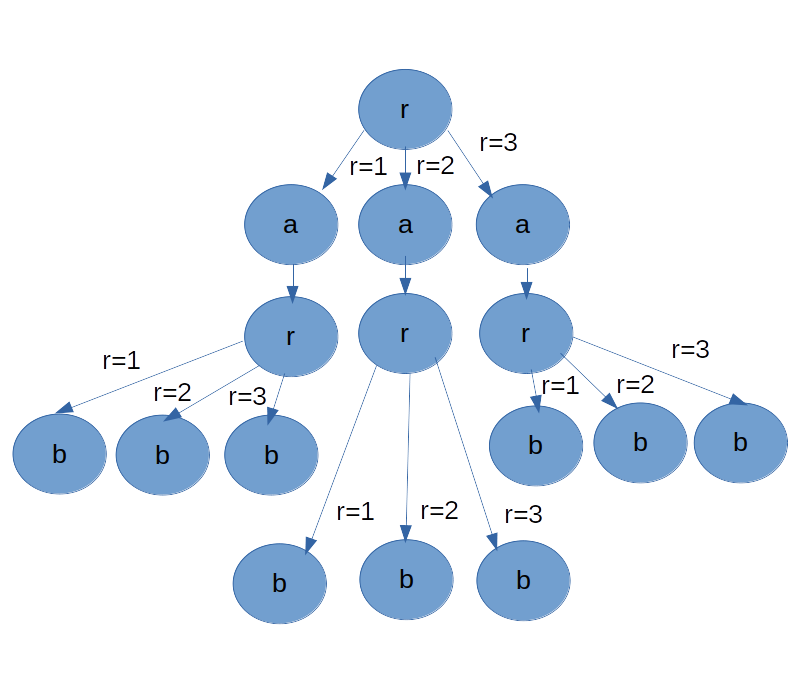
\includegraphics[width=0.7\linewidth]{Graphics/Neigh-Tree}
	\caption{Árbol de vecindad asociado a $rarb$.}
	\label{fig:neigh-tree}
\end{figure}

Cada rama del árbol representa un conjunto de soluciones vecinas. Por ejemplo, en la figura \ref{fig:neigh-tree}, la rama más a la izquierda representa todas las posibles soluciones en las que el cliente se escoge de la primera ruta y se inserta también en la primera ruta.

A partir del árbol que representa a una vecindad para una solución, es posible contar la cantidad de vecinos y es posible asignarle a cada vecino un número natural \cite{Hector}. De esta manera, explorar una vecindad se reduce a seleccionar elementos de los $n$ primeros números. En una exploración exhaustiva se seleccionan todos los números mientras que en una aleatoria se selecciona sólo un conjunto de ellos. Usando esta idea, las estrategias de exploración se definen como iteradores que generan un número, calculan cuál es la solución que le corresponde y retornan esta solución en forma de lista de operaciones.

El Árbol de Vecindad permite explorar vecinos. Para cada vecino se necesita conocer su costo y en la siguiente sección se muestra cómo se pueden obtener estos costos mediante un Grafo de Evaluación.

\section{Grafo de Evaluación}\label{1-JJ}
Para resolver un VRP utilizando búsqueda local, es necesario obtener el costo de cada vecino. Los algoritmos de búsqueda local obtienen un vecino a partir de pequeñas modificaciones de la solución actual. Calcular el costo del vecino evaluando la solución en su totalidad suele ser menos eficiente que calcular la variación del costo debido a las operaciones. Por eso, al programar estos algoritmos, es conveniente determinar la manera más eficiente de evaluar vecinos con la menor cantidad de operaciones posibles. 

Por ejemplo, en CVRP, al eliminar un cliente de una ruta sólo es necesario calcular la nueva distancia a partir de la eliminación, y modificar la carga que debe tener el vehículo a lo largo de la ruta. Algo similar ocurre cuando se inserta un cliente.

Si se desea obtener el costo de un vecino con la menor cantidad de operaciones posible, para cada problema y cada operación del criterio de vecindad, se debe programar sus diferencias. Esto puede variar mucho de un problema a otro por lo que calcular el costo de un vecino, para cada variante de VRP es un trabajo distinto y necesita una implementación diferente.

Por ejemplo, en CVRP sólo se debe actualizar la distancia recorrida y la capacidad restante del vehículo, pero en un problema con \textit{backhaul} hay que verificar también si no se incumple la restricción de que todos los clientes de tipo A se visiten antes de los de tipo B.  

Este es, precisamente, uno de los motivos por el que resolver un Problema de Enrutamiento de Vehículos requiere tiempo de desarrollo humano, al tener que programar cómo calcular el costo de los vecinos para cada nuevo problema. En \cite{JJ} se propone un mecanismo que permite calcular el costo de cualquier vecino, a partir, únicamente, del código que calcula el costo de una solución inicial. Esto se hace a través de un Grafo de Evaluación que se expone a continuación.

El Grafo de Evaluación es una estructura que permite almacenar las operaciones realizadas durante la evaluación de una solución. En este grafo hay tres tipos de nodos:

\begin{itemize}
	\item Nodos que representan los elementos de la solución (clientes, depósitos).
	\item Nodos que representan variables y mantienen sus valores (como el costo total). Estos se denominan nodos acumuladores.
	\item Nodos que representan las operaciones involucradas en una evaluación (aumentar valor, disminuir valor). Estos se denominan nodos operacionales.
\end{itemize}

Para calcular el costo de un vecino a partir de las operaciones que se necesitan para obtenerlo, el grafo se modifica para reflejar las modificaciones que se hicieron sobre la solución. El Grafo de Evaluación permite obtener costos de soluciones vecinas de una solución actual de forma eficiente, ya que garantiza que sólo se recalculen los fragmentos de las nuevas soluciones en los que estas se diferencien de la solución actual.

En las siguientes secciones se muestra cómo construir el grafo y cómo ejecutar operaciones sobre un grafo construido .

\subsection{Creación del grafo}

Para construir el grafo, primero se inicializa con los nodos que representan elementos de la solución. Por ejemplo, en la figura \ref{fig:eval-graph-1} se muestra el grafo inicializado con los nodos que representan los elementos de la solución: $s = [(c_1,c_2), (c_3,c_4)]$. Los nodos \textit{d} representan al depósito y los nodos \textit{$c_i$} a cada cliente. Todas las rutas en el grafo comienzan y terminan con nodos depósito.

Luego, el usuario debe ejecutar el código de evaluación de la variante específica que se quiere resolver y, a partir de este código, se construyen los nodos acumuladores y los nodos operacionales. Por ejemplo, a continuación se muestra el código de evaluación de VRP básico en el que soólo se calcula la distancia recorrida:

\begin{lstlisting}
def-var total-distance as 0
loop for r in solution-routes do
	loop for c in r-clients do
		increment total-distance with distance between r-previous-client and c
	set previous-client as c
return-value total-distance graph
\end{lstlisting}

En la línea 1 se crea un nodo para mantener el valor del costo total y en la línea 4 se crean los nodos que aumentan el valor de la distancia total. Cómo programar códigos de evaluación se explicará detalladamente en la sección \ref{2-eval}.

\begin{figure}
	\centering
	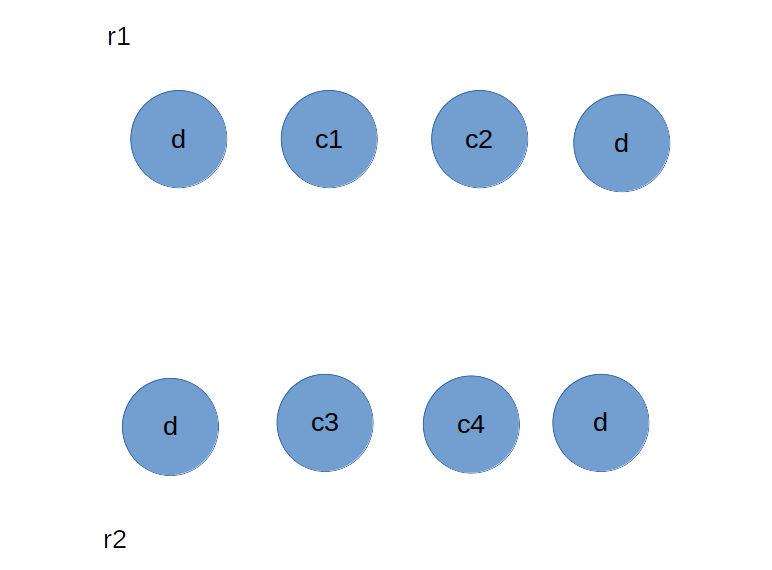
\includegraphics[width=0.9\linewidth]{Graphics/graph-init}
	\caption{Nodos que representan elementos de la solución $s_1$ de VRP básico.}
	\label{fig:eval-graph-1}
\end{figure}

Cuando se ejecuta el código de evaluación a la solución con la que se inicializó el grafo de la figura \ref{fig:eval-graph-1}, se le agregan a este los nodos operacionales y acumuladores. Entonces se obtiene el grafo representado en la figura \ref{fig:eval-graph-2}. El nodo \textit{cost} almacena el costo total de la solución y los nodos con símbolo \textit{+} son nodos operacionales que toman como entrada dos nodos clientes (o depósito) y adicionan al nodo de costo total la distancia entre ellos.

\begin{figure}
	\centering
	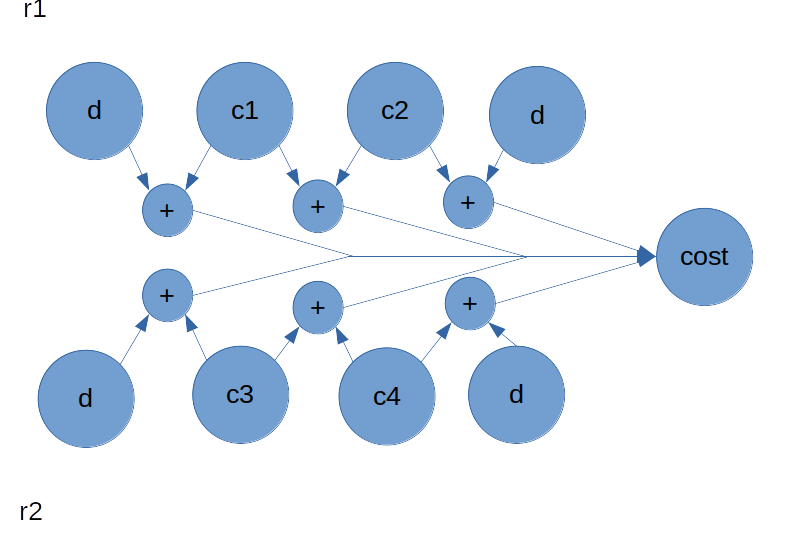
\includegraphics[width=0.9\linewidth]{Graphics/eval-graph-2}
	\caption{Grafo de evaluación que representa la solución $s1$ de VRP básico.}
	\label{fig:eval-graph-2}
\end{figure}

\subsection{Modificación del grafo}
Una vez construido el grafo, las modificaciones que se le realizan se definen mediante operaciones elementales (como eliminar o insertar cliente). Cuando se agregan o eliminan nodos que representan elementos de la solución, se modifican todos los nodos operacionales que dependen de ellos. Estos nodos operacionales tienen asociadas funciones para ejecutarse y para deshacerse. 

Por ejemplo, retirar el cliente $c1$ del grafo representado en \ref{fig:eval-graph-2} (VRP clásico) provoca que los dos nodos \textit{+} que utilizan dicho cliente como entrada deshagan sus operaciones, y al mismo tiempo, se crea y ejecuta un nuevo nodo \textit{+} que recibe como entrada $d$ y $c2$. Luego, insertar a $c1$ al final de la ruta $r2$ se deshace la operación el nodo \textit{+} que recibe como entrada a $c4$ y $d$ mientras se crean y ejecutan dos nodos \textit{+} nuevos, uno recibiendo de entrada a $c4$ y $c1$ mientras que el otro a $c1$ y $d$. El resultado de estas dos operaciones se muestra en \ref{fig:eval-graph-4} y es, precisamente, el grafo resultante de aplicar al grafo de la figura \ref{fig:eval-graph-2}, el criterio \texttt{mover un cliente a cualquier ruta en cualquier posición}, formado por las siguientes operaciones:

\begin{itemize}
	\item Seleccionar ruta \texttt{r1}.
	\item Seleccionar cliente \texttt{c1} de la posición \texttt{2} de la ruta \texttt{r1}.
	\item Seleccionar ruta \texttt{r2}.
	\item Insertar cliente \texttt{c1} en la posición texttt{3} de la ruta \texttt{r2}.
\end{itemize}

Nótese que luego de aplicar los métodos \texttt{evaluate} y \texttt{undo} correspondientes el nodo $cost$ tiene almacenado el costo de la solución resultante luego de aplicar el criterio \texttt{mover cliente a una posición aleatoria en una ruta aleatoria}. Para encontrar el costo de la nueva solución sólo fue necesario analizar y modificar los nodos en que el grafo de la solución nueva se diferencia de la solución anterior y no todo el grafo. En esto se basa la evaluación \textit{eficiente} del Grafo de Evaluación.

\begin{figure}
	\centering
	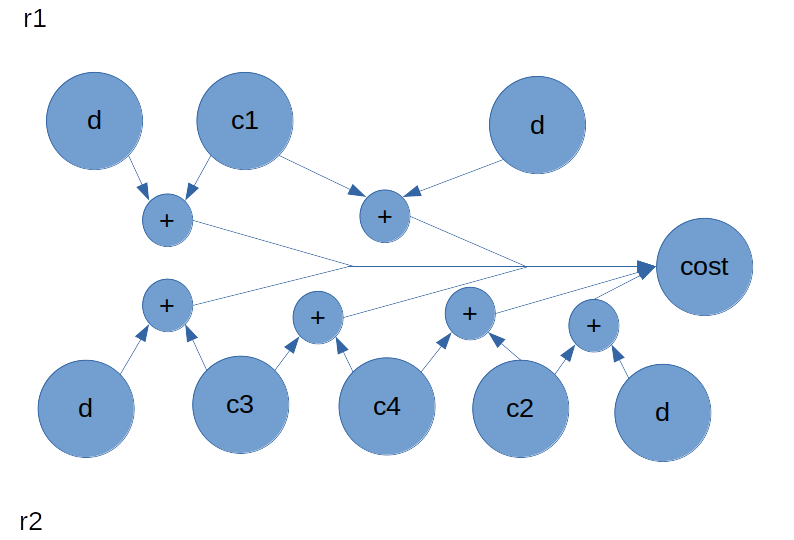
\includegraphics[width=0.9\linewidth]{Graphics/eval-graph-4}
	\caption{Grafo de evaluación que representa la solución $s1$ de VRP básico luego de mover el cliente $c2$}
	\label{fig:eval-graph-4}
\end{figure}

Para explorar una vecindad a partir de un criterio es necesario (además de generar y evaluar soluciones) decidir e implementar estrategias de exploración y de selección. A partir de combinaciones de diferentes estrategias se pueden realizar exploraciones con distintos resultados. Esto se trata en la siguiente sección.

\section{Combinación de estrategias de exploración y selección.}\label{1-Heidy}
Las exploraciones de las vecindades obtienen diferentes resultados en dependencia de las estrategias de exploración y de selección que se utilice. Por ejemplo, a partir de una solución actual y un criterio, se puede explorar una vecindad con una búsqueda exhaustiva y mejora aleatoria o con una búsqueda aleatoria y primera mejora. En ambos casos se pueden encontrar soluciones distintas. Programar cada combinación de estas estrategias demanda tiempo de trabajo humano.

En \cite{Heidy} se propone una herramienta que permite generar funciones de exploración a partir de un criterio, una estrategia de selección y una de exploración. Las posibles estrategias se definen como clases y usando instancias de estas clases se puede generar una función de exploración que se comporte de acuerdo a las instancias recibidas. La generación de cada porción del código se logra utilizando funciones genéricas, en particular los métodos \texttt{after} \cite{Lisp2006}.

La función de exploración resultante recibe el problema que se quiere resolver junto con una solución actual, ejecuta la exploración y retorna un vecino de acuerdo al criterio de selección. Si ninguna solución explorada cumple con la estrategia de selección, se retorna \texttt{nil}. 

En \cite{Heidy}, para realizar la exploración, se utilizaban ciclos que hacían poco flexible incorporar nuevas estrategias. Con el Árbol de vecindad es posible crear cualquier exploración y diseñar estrategias de búsqueda más complejas. Además, en \cite{Heidy} tampoco se usa el Grafo de Evaluación por lo que la cantidad de problemas que podían ser evaluados era limitada. En este trabajo se combinan el Árbol de Vecindad y el Grafo de Evaluación junto con el generador de funciones de exloración. Esto permite resolver cualquier problema que se pueda evaluar en el grafo, con cualesquiera combinaciones de estrategias de exploración y selección. El siguiente capítulo expone cómo se unen todas estas herramientas.





























